\chapter{Advanced Cryptographic Primitives}
\label{ch:advanced-primitives}

\abstract*{Lattice-based cryptography enables capabilities far beyond encryption and signatures.  This chapter introduces fully homomorphic encryption, zero-knowledge proofs, and secure multiparty computation---primitives that were theoretical curiosities until lattice theory made them practical.  The noise dynamics of LWE-based schemes play a central role: noise growth constrains what can be computed homomorphically, and the techniques for managing it---modulus switching, bootstrapping, careful parameter selection---reappear in different guises across all three primitives.  The chapter closes with a survey of lattice-based advanced constructions---attribute-based encryption, identity-based encryption, threshold signatures, and functional encryption---that point toward a richer cryptographic future.}

\abstract{Lattice-based cryptography enables capabilities far beyond encryption and signatures.  This chapter introduces fully homomorphic encryption, zero-knowledge proofs, and secure multiparty computation---primitives that were theoretical curiosities until lattice theory made them practical.  The noise dynamics of LWE-based schemes play a central role throughout, and the techniques for managing noise reappear in different guises across all three primitives.  The chapter closes with a survey of lattice-based advanced constructions that point toward a richer cryptographic future.}

% =============================================================
% SOURCE: notes.tex §6.2 (lines 8327–8905)
% REUSE: ~40%.  Good overviews with physics analogies.
% Keep focused — this is a gateway chapter, not a treatise.
% =============================================================


\section{Fully Homomorphic Encryption}
\label{sec:fhe}

Imagine encrypting your medical records before uploading them to the cloud, having the cloud run a diagnostic algorithm on that encrypted data, and receiving encrypted results that only you can decrypt.  The cloud processes your data faithfully yet learns nothing about it.  This seemingly impossible capability---\emph{fully homomorphic encryption} (FHE)\index{fully homomorphic encryption}---has moved from theoretical breakthrough to practical deployment in under two decades, powered by the same lattice problems that underpin post-quantum security.

\subsection{The Concept: Computing on Encrypted Data}
\label{subsec:fhe-concept}

\begin{definition}[Homomorphic Encryption]
\label{def:fhe}
An encryption scheme $(\Gen, \Enc, \Dec, \mathsf{Eval})$ is \emph{fully homomorphic}\index{FHE|see{fully homomorphic encryption}} if it supports an efficient evaluation algorithm $\mathsf{Eval}$ such that for any circuit $f$ and any plaintexts $m_1, \ldots, m_k$:
\begin{equation}
\label{eq:fhe-correctness}
\Dec\bigl(\mathit{sk},\; \mathsf{Eval}(f,\, \Enc(\mathit{pk}, m_1),\, \ldots,\, \Enc(\mathit{pk}, m_k))\bigr) \;=\; f(m_1, \ldots, m_k),
\end{equation}
where $\mathsf{Eval}$ works without access to the secret key $\mathit{sk}$.
\end{definition}

It suffices that $\mathsf{Eval}$ supports addition and multiplication of ciphertexts, since these two operations are \emph{universal}---any Boolean or arithmetic circuit can be built from them.  Schemes supporting only one operation (e.g., unpadded RSA is multiplicatively homomorphic) are called \emph{partially homomorphic}; schemes supporting both but only to a bounded depth are called \emph{somewhat homomorphic} (SHE).

\begin{svgraybox}
\textbf{Why FHE matters.}
Public-key encryption protects data \emph{at rest} and \emph{in transit}.  FHE protects data \emph{in use}.  This is the missing piece for privacy-preserving cloud computing: a hospital can outsource genomic analysis, a bank can outsource fraud detection, and a government can outsource census statistics---all without exposing raw data to the computing party.
\end{svgraybox}

Figure~\ref{fig:ch14-fhe-cloud} summarises the FHE workflow: a client encrypts private data, a cloud server computes on the ciphertext without ever seeing the plaintext, and the client decrypts the result to obtain the output of the computation.

\begin{figure}[t]
\centering
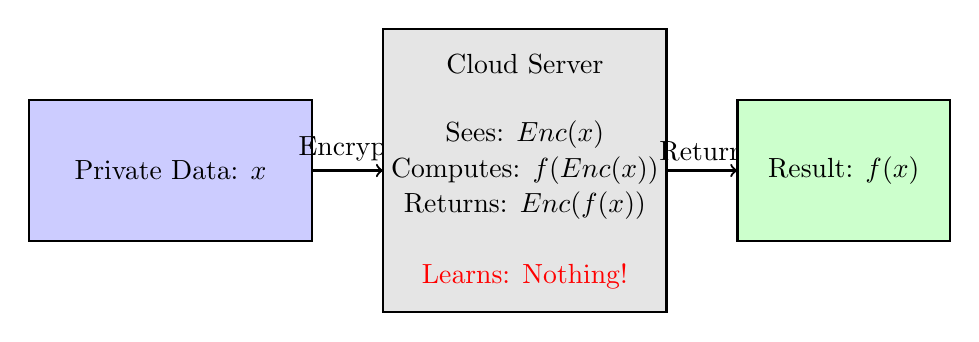
\begin{tikzpicture}[scale=0.9]
    % Client side
    \draw[thick, fill=blue!20] (-2,-1) rectangle (2,1);
    \node at (0,0) {Private Data: $x$};

    % Encryption
    \draw[->, thick] (2,0) -- (3,0);
    \node[above] at (2.5,0) {Encrypt};

    % Cloud
    \draw[thick, fill=gray!20] (3,-2) rectangle (7,2);
    \node at (5,1.5) {Cloud Server};
    \node at (5,0.5) {Sees: $Enc(x)$};
    \node at (5,0) {Computes: $f(Enc(x))$};
    \node at (5,-0.5) {Returns: $Enc(f(x))$};
    \node[red] at (5,-1.5) {Learns: Nothing!};

    % Return
    \draw[->, thick] (7,0) -- (8,0);
    \node[above] at (7.5,0) {Return};

    % Decryption
    \draw[thick, fill=green!20] (8,-1) rectangle (11,1);
    \node at (9.5,0) {Result: $f(x)$};
\end{tikzpicture}
\caption{Fully homomorphic encryption: computing on encrypted data without decryption.  The cloud processes ciphertexts and returns an encrypted result, learning nothing about the underlying data.}
\label{fig:ch14-fhe-cloud}
\end{figure}


\subsection{Gentry's Blueprint: Somewhat HE Plus Bootstrapping}
\label{subsec:gentry-blueprint}

The existence of FHE was an open problem for over 30~years, from Rivest, Adleman, and Dertouzos's 1978 conjecture to Gentry's 2009 resolution~\cite{Gentry2009}.  Gentry's construction follows a two-step blueprint that remains the template for all modern FHE schemes:

\begin{enumerate}
\item \textbf{Build a somewhat homomorphic scheme.}  Construct an encryption scheme that supports both homomorphic addition and multiplication, but only for circuits up to some bounded depth~$L$.

\item \textbf{Bootstrap to full homomorphism.}  Use the SHE scheme to homomorphically evaluate its \emph{own decryption circuit}, thereby ``refreshing'' a noisy ciphertext into a fresh one.  If the decryption circuit has depth less than~$L$, one application of $\mathsf{Eval}$ resets the noise without exceeding the scheme's capacity, and the process can be repeated indefinitely.
\end{enumerate}

The bootstrapping step is the conceptual leap.  The evaluator encrypts the secret key under the public key (a so-called \emph{bootstrapping key}), then homomorphically computes decryption ``inside the encryption.''  The output is a fresh ciphertext of the same plaintext, with noise reset to the level introduced by one decryption-circuit evaluation.

At first glance, bootstrapping seems to violate a basic principle: computation on noisy data should only increase the noise, never reduce it.  The resolution is that noise is not destroyed---it is \emph{paid for}.  The bootstrapping procedure decrypts and re-encrypts homomorphically, and the computational cost of doing so (time, memory, ciphertext expansion) is the price of resetting the noise floor.  The bookkeeping is exact: any circuit of depth~$D$ that would otherwise require a modulus $q$ exponential in~$D$ can instead use a polynomial modulus at the cost of $D/L$ bootstrapping operations, each with latency proportional to the decryption-circuit depth.  Nothing is free; the noise budget is traded for a time budget.


\subsection{LWE-Based FHE: BGV, BFV, CKKS, and TFHE}
\label{subsec:fhe-schemes}

All modern FHE schemes derive their security from the Learning With Errors problem (Chap.~\ref{ch:lwe-encryption}) or its ring/module variants~\cite{Regev2009}.  They share a common algebraic skeleton---a ciphertext is an \lwe{} (or Ring-\lwe{}) sample $(\mathbf{a}, b = \ip{\mathbf{a}}{\mathbf{s}} + e + \Delta m)$ where $\Delta$ is an encoding factor and $e$ is the noise term---but they differ in two fundamental design choices: how plaintexts are encoded and how noise is kept under control.

BGV and BFV both operate over integers modulo a prime~$p$, making them natural choices for exact integer arithmetic.  They diverge in noise management: BGV uses \emph{modulus switching}, progressively shrinking the ciphertext modulus after each multiplication to reduce the relative noise, while BFV adopts a \emph{scale-invariant} approach that keeps the modulus fixed and instead manages the ratio between signal and noise through careful encoding.  CKKS takes a fundamentally different path by encoding approximate real numbers---accepting small rounding errors in the plaintext in exchange for native support of floating-point workloads such as machine learning and statistics.  TFHE occupies the opposite extreme, encrypting single bits and evaluating Boolean circuits gate by gate, but compensating with extremely fast bootstrapping (sub-millisecond on modern hardware) that resets noise after every gate.  Table~\ref{tab:fhe-schemes} summarises these families.

\begin{table}[t]
\caption{Modern FHE scheme families and their characteristics}
\label{tab:fhe-schemes}
\begin{tabular}{p{2cm}p{3.5cm}p{3cm}p{3cm}}
\hline\noalign{\smallskip}
\textbf{Scheme} & \textbf{Plaintext space} & \textbf{Best for} & \textbf{Noise management} \\
\noalign{\smallskip}\svhline\noalign{\smallskip}
BGV & Integers mod $p$ & Exact integer arithmetic & Modulus switching \\
BFV & Integers mod $p$ & Exact integer arithmetic & Scale-invariant \\
CKKS & Approximate reals & Machine learning, statistics & Rescaling \\
TFHE & Single bits & Boolean circuits, fast bootstrap & Gate bootstrapping \\
\noalign{\smallskip}\hline
\end{tabular}
\end{table}

Despite these differences, the four families share the same fundamental bottleneck.  Homomorphic addition adds two \lwe{} samples and the noise grows additively; homomorphic multiplication involves a tensor product that causes the noise to grow \emph{multiplicatively}.  This multiplicative noise growth is what limits the depth of circuits that can be evaluated without bootstrapping, and managing it is the central challenge of every FHE implementation.


\subsection{Noise Growth and the Depth Barrier}
\label{subsec:noise-growth}

The central constraint on any LWE-based FHE scheme is noise growth.  Every homomorphic operation increases the noise in the ciphertext, and once the noise exceeds a threshold, decryption fails.  Understanding the precise rate of growth is essential for choosing parameters and deciding when bootstrapping is needed.

\begin{definition}[Noise Budget]
\label{def:noise-budget}
A fresh ciphertext in an \lwe{}-based scheme carries a noise term $e$ with magnitude $\norm{e} \approx \sigma$.  After homomorphic operations, the noise evolves as:
\begin{align}
\text{Addition:}\quad & \norm{e_{\mathrm{add}}} \;\approx\; \norm{e_1} + \norm{e_2}, \label{eq:noise-add}\\
\text{Multiplication:}\quad & \norm{e_{\mathrm{mult}}} \;\approx\; \norm{e_1}\cdot\norm{e_2}\cdot\poly(n). \label{eq:noise-mult}
\end{align}
Decryption fails when $\norm{e} \geq q/2$, where $q$ is the ciphertext modulus.  The \emph{noise budget} is $\log_2(q / 2\norm{e})$ bits.
\end{definition}

Equation~\eqref{eq:noise-mult} is the crux: after $L$ levels of multiplication, noise grows as $\sigma^{2^L}\cdot\poly(n)^L$.  Without intervention, even modest circuits exhaust the noise budget.

The analogy to signal processing is precise, not merely suggestive.  In a chain of analog amplifiers, each stage adds thermal noise and amplifies the noise from all previous stages; after $L$ stages the signal-to-noise ratio degrades exponentially.  The standard engineering solution is a \emph{regenerative repeater}: decode the analog signal to digital, then re-encode it, resetting the noise floor at the cost of latency.  FHE bootstrapping does exactly this---it homomorphically decrypts (decodes) and re-encrypts (re-encodes), resetting noise at the cost of computational latency.  The parallel is structural, not metaphorical: both systems face exponential noise growth from iterated nonlinear operations, and both solve it by interleaving decode-reencode steps.  The difference is that in FHE the ``decoding'' itself must happen on encrypted data, which is why bootstrapping is so expensive.


\subsection{Bootstrapping: The Noise Reset}
\label{subsec:bootstrapping}

Bootstrapping is the operation that transforms somewhat homomorphic encryption into \emph{fully} homomorphic encryption.  Given a ciphertext $c$ with high noise, bootstrapping produces a ciphertext $c'$ encrypting the same plaintext with low noise:

\begin{enumerate}
\item Publish an encrypted secret key: $\widetilde{\mathit{sk}} = \Enc(\mathit{pk}, \mathit{sk})$.
\item Homomorphically evaluate the decryption function: $c' \leftarrow \mathsf{Eval}(\Dec(\cdot, \widetilde{\mathit{sk}}),\; c)$.
\item The output $c'$ is a fresh encryption of the original plaintext $m$, with noise determined only by the depth of the decryption circuit.
\end{enumerate}

The circular-security assumption---that it is safe to encrypt the secret key under its own public key---is required but widely believed to hold for \lwe{}-based schemes.

\begin{example}[Bootstrapping Cost Over Time]
\label{ex:bootstrap-progress}
The practical viability of FHE is measured by bootstrapping speed.  Gentry's original scheme required approximately 30~minutes per bootstrap in 2009.  TFHE reduced this to 13~ms by 2016, and current GPU-accelerated implementations achieve sub-millisecond bootstraps.  This six-orders-of-magnitude improvement in 15~years has brought FHE from theoretical curiosity to deployable technology.
\end{example}


\subsection{Practical FHE Today}
\label{subsec:fhe-practice}

Several open-source libraries have brought FHE from research papers to production code.  Microsoft SEAL implements BFV and CKKS and has become the de facto platform for privacy-preserving machine learning, with bindings in C++, .NET, and Python.  TFHE-rs, developed by Zama, implements TFHE with fast gate bootstrapping and targets Boolean circuits and integer operations where per-gate refresh is essential.  OpenFHE provides a unified API spanning BGV, BFV, CKKS, and TFHE, making it possible to prototype across scheme families within a single codebase and select the best fit for a given workload.

\begin{example}[Private Medical Diagnosis]
\label{ex:fhe-medical}
A hospital encrypts a patient's genomic data (approximately 3~GB) and uploads it to a cloud server.  The cloud homomorphically evaluates a cancer risk model---comparing one million single-nucleotide polymorphisms---and returns encrypted risk scores.  The hospital decrypts the result; the cloud learns nothing about the patient.  Current systems perform this computation in a few hours on commodity hardware, at a fraction of the cost of building an in-house secure computation facility.
\end{example}


%% ================================================================
\section{Zero-Knowledge Proofs}
\label{sec:zkp}

A zero-knowledge proof\index{zero-knowledge proof} allows a \emph{prover} to convince a \emph{verifier} that a statement is true, without revealing \emph{any} information beyond the truth of the statement itself.  This paradoxical-sounding capability is one of the most powerful ideas in modern cryptography.

\subsection{The Concept: Proving Without Revealing}
\label{subsec:zkp-concept}

\begin{definition}[Zero-Knowledge Proof]
\label{def:zkp}
An interactive protocol between a prover~$P$ and a verifier~$V$ for a language $\mathcal{L}$ satisfies three properties:
\begin{itemize}
\item \textbf{Completeness:} If $x \in \mathcal{L}$, the honest prover convinces the verifier with probability~$1$ (or $1 - \negl(\lambda)$).
\item \textbf{Soundness:} If $x \notin \mathcal{L}$, no cheating prover convinces the verifier except with probability $\negl(\lambda)$.
\item \textbf{Zero-knowledge:} The verifier's view can be \emph{simulated} without interaction with the prover.  Formally, there exists a polynomial-time simulator $S$ such that $S(x) \approx \mathrm{View}_V(P \leftrightarrow V)(x)$.
\end{itemize}
\end{definition}

The zero-knowledge property is the remarkable one: the verifier learns that ``$x \in \mathcal{L}$'' but gains no additional knowledge---not even a single bit about \emph{why} the statement is true.

The zero-knowledge property has a flavour that readers with a physics background may recognise.  Measuring a qubit in the computational basis yields one bit and irreversibly collapses the state, destroying access to all other information the qubit encoded.  A zero-knowledge proof achieves something analogous by design rather than physics: the verifier receives exactly one bit of information---``the statement is true''---and the simulator argument guarantees, mathematically, that no additional information can be extracted.  The mechanisms are entirely different (cryptographic simulation versus quantum collapse), but the operational consequence is the same: a hard, provable bound on what the receiving party can learn.

A classical illustration of this concept is the graph 3-colorability protocol, shown in Figure~\ref{fig:ch14-zk-coloring}.  The prover knows a valid 3-coloring of a graph and convinces the verifier of this fact by repeatedly committing to a random recoloring (a permutation of the colors), letting the verifier pick an edge, and revealing only the two endpoint colors.  After sufficiently many rounds the verifier is convinced the coloring is valid, yet has learned nothing about the actual coloring itself.

\begin{figure}[t]
\centering
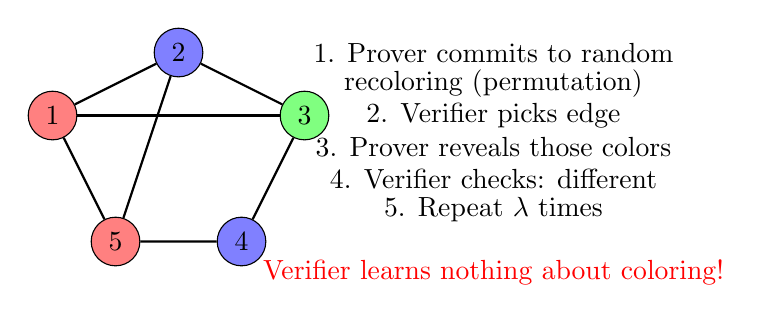
\begin{tikzpicture}[scale=0.8]
    % Graph
    \node[circle, draw, fill=red!50] (1) at (0,2) {1};
    \node[circle, draw, fill=blue!50] (2) at (2,3) {2};
    \node[circle, draw, fill=green!50] (3) at (4,2) {3};
    \node[circle, draw, fill=blue!50] (4) at (3,0) {4};
    \node[circle, draw, fill=red!50] (5) at (1,0) {5};

    % Edges
    \draw[thick] (1) -- (2) -- (3) -- (4) -- (5) -- (1);
    \draw[thick] (1) -- (3);
    \draw[thick] (2) -- (5);

    % Protocol
    \node[align=left] at (7,3) {1. Prover commits to random};
    \node[align=left] at (7,2.5) {recoloring (permutation)};
    \node[align=left] at (7,2) {2. Verifier picks edge};
    \node[align=left] at (7,1.5) {3. Prover reveals those colors};
    \node[align=left] at (7,1) {4. Verifier checks: different};
    \node[align=left] at (7,0.5) {5. Repeat $\lambda$ times};

    \node[red] at (7,-0.5) {Verifier learns nothing about coloring!};
\end{tikzpicture}
\caption{Zero-knowledge proof of graph 3-colorability: the prover demonstrates knowledge of a valid coloring without revealing it, by committing to random permutations and revealing only queried edges.}
\label{fig:ch14-zk-coloring}
\end{figure}


\subsection{Interactive Proofs and the Fiat--Shamir Heuristic}
\label{subsec:fiat-shamir}

The classical structure of an interactive zero-knowledge proof follows a three-move \emph{sigma protocol}\index{sigma protocol}:

\begin{enumerate}
\item \textbf{Commitment.} The prover sends a commitment $a$ (e.g., a randomised encryption).
\item \textbf{Challenge.} The verifier sends a random challenge $c \getsr \{0,1\}^\lambda$.
\item \textbf{Response.} The prover sends a response $z$ that the verifier checks against $(a, c)$.
\end{enumerate}

To eliminate interaction, Fiat and Shamir~\cite{FiatShamir1986} proposed replacing the verifier's random challenge with the output of a cryptographic hash function applied to the commitment and the statement:
\begin{equation}
\label{eq:fiat-shamir}
c \;=\; H(a \,\|\, x),
\end{equation}
where $H$ is modelled as a random oracle\index{random oracle}.  The resulting \emph{non-interactive} proof $\pi = (a, z)$ can be verified by anyone, without live interaction.

\begin{definition}[Post-Quantum Fiat--Shamir Security]
\label{def:pq-fiat-shamir}
In the quantum random oracle model (QROM)\index{QROM}, the Fiat--Shamir transform remains sound but incurs a security loss: an adversary making $q$ quantum queries to $H$ achieves soundness error $\bigO(\sqrt{q} \cdot \varepsilon)$ rather than $\varepsilon$, where $\varepsilon$ is the soundness error of the interactive protocol.  This $\sqrt{q}$ factor must be accounted for when setting security parameters.
\end{definition}

The Fiat--Shamir transform is the mechanism behind the CRYSTALS-Dilithium (ML-DSA) signature scheme (Chap.~\ref{ch:lattice-signatures}).


\subsection{Lattice-Based Zero-Knowledge: Stern-Type Protocols}
\label{subsec:lattice-zk}

Lattices enable efficient zero-knowledge proofs for algebraically structured statements.  The prototypical example is \emph{proving knowledge of a short vector}:

\begin{example}[ZK Proof of a Short Preimage]
\label{ex:stern-proof}
\textbf{Statement:} ``I know $\mathbf{s} \in \Z^m$ with $\norm{\mathbf{s}} \leq \beta$ such that $\mathbf{A}\mathbf{s} = \mathbf{t} \pmod{q}$.''

A Stern-type protocol\index{Stern protocol} proceeds as follows:
\begin{enumerate}
\item \textbf{Commit:} Sample a mask $\mathbf{y} \getsr D_{\Z^m, \sigma}$ (discrete Gaussian) and send $\mathbf{w} = \mathbf{A}\mathbf{y} \pmod{q}$.
\item \textbf{Challenge:} Receive a random challenge $c \in \{0, 1, 2\}$.
\item \textbf{Respond:}
  \begin{itemize}
  \item If $c = 0$: reveal $\mathbf{y}$ and $\mathbf{s}$ in permuted form.
  \item If $c = 1$: reveal $\mathbf{z} = \mathbf{y} + \mathbf{s}$ and a commitment opening.
  \item If $c = 2$: reveal $\mathbf{y}$ and a commitment to $\mathbf{s}$.
  \end{itemize}
\item \textbf{Verify:} Check the appropriate linear relation and norm bound.
\end{enumerate}
Each round has soundness error $2/3$.  After $\lambda$ rounds, the soundness error drops to $(2/3)^\lambda$, which is negligible for $\lambda \approx 200$.  The mask $\mathbf{y}$ information-theoretically hides the secret $\mathbf{s}$, provided $\sigma$ is large enough relative to $\norm{\mathbf{s}}$.
\end{example}

Stern-type proofs are the basis of several post-quantum anonymous credential schemes and group signature proposals.


\subsection{Post-Quantum SNARKs and STARKs}
\label{subsec:snarks-starks}

\emph{Succinct Non-interactive Arguments of Knowledge} (SNARKs)\index{SNARK} compress proofs to a few hundred bytes and enable verification in milliseconds, regardless of the complexity of the proven statement.  Most deployed SNARKs rely on elliptic-curve pairings and are therefore vulnerable to quantum attack.

Two post-quantum alternatives have emerged, pursuing different trade-offs.  \textbf{STARKs}\index{STARK} (Scalable Transparent Arguments of Knowledge) replace pairings entirely with hash-based polynomial commitments.  The resulting proofs are larger---tens of kilobytes rather than hundreds of bytes---but they rely only on collision-resistant hash functions, which are already quantum-safe, and they require no trusted setup.  This transparency is a significant practical advantage: there is no toxic waste, no multi-party ceremony, and no trust assumption beyond the hash function itself.

\textbf{Lattice-based SNARKs} take the opposite approach, replacing pairing-based polynomial commitments with lattice-based ones while preserving the algebraic structure that makes SNARKs succinct.  Active research has produced proof sizes in the range of 10--50~KB with verification times around 100~ms---competitive with STARKs in size, but with the added benefit of richer algebraic operations.  The main challenge is prover time, which can be orders of magnitude slower than pairing-based provers due to the overhead of lattice arithmetic.

\begin{table}[t]
\caption{Comparison of proof systems for post-quantum zero-knowledge}
\label{tab:pq-zk}
\begin{tabular}{p{3cm}p{2.5cm}p{2.5cm}p{3.5cm}}
\hline\noalign{\smallskip}
\textbf{System} & \textbf{Proof size} & \textbf{Verification} & \textbf{Assumption} \\
\noalign{\smallskip}\svhline\noalign{\smallskip}
Classical SNARK & $\sim$128 bytes & $\sim$10 ms & Pairings (quantum-broken) \\
STARK & 10--200 KB & $\sim$50 ms & Hash functions \\
Lattice SNARK & 10--50 KB & $\sim$100 ms & \lwe{} / \textsc{SIS} \\
Stern-type & $\sim$100 KB & $\sim$200 ms & \lwe{} / \textsc{SIS} \\
\noalign{\smallskip}\hline
\end{tabular}
\end{table}


\subsection{Applications of Zero-Knowledge}
\label{subsec:zk-applications}

Zero-knowledge proofs underpin a surprisingly wide range of privacy-preserving applications.  In \emph{anonymous authentication}, a user proves membership in a group---``I hold a valid credential issued by this authority''---without revealing which credential, enabling systems where identity verification does not require identity disclosure.  \emph{Range proofs} allow a party to demonstrate that a private value lies in an interval (``my account balance exceeds the required minimum'') without revealing the value itself; these are essential in financial compliance, where regulations demand verification but privacy law demands confidentiality.  \emph{Verifiable computation} inverts the trust model of cloud outsourcing: instead of trusting the server, a client receives a proof that the computation was executed correctly, turning trust into mathematics.  Finally, zero-knowledge proofs are the engine behind privacy-preserving blockchains, where transaction validity must be publicly verifiable even though sender, receiver, and amount remain hidden.

Each of these applications currently relies on pre-quantum proof systems.  As the transition to post-quantum cryptography proceeds, they will need quantum-safe instantiations---making the lattice-based and hash-based proof systems discussed above not just theoretically interesting but practically urgent.


%% ================================================================
\section{Secure Multiparty Computation}
\label{sec:mpc}

In secure multiparty computation (MPC)\index{multiparty computation}, $n$ parties holding private inputs $x_1, \ldots, x_n$ jointly compute a function $f(x_1, \ldots, x_n)$ such that each party learns the output but nothing else about the other parties' inputs---even if some parties are corrupted.

\subsection{The Millionaires' Problem}
\label{subsec:millionaires}

Yao's \emph{millionaires' problem}\index{millionaires' problem} (1982) is the canonical MPC example: Alice and Bob each know their net worth and wish to determine who is richer without revealing the actual amounts.  The problem generalises immediately: any function computable by a circuit can be evaluated securely by multiple parties.  Figure~\ref{fig:ch16-mpc} illustrates the essential guarantee: the protocol reveals only the comparison result, while each party's private input remains hidden from the other.

\begin{figure}[t]
\centering
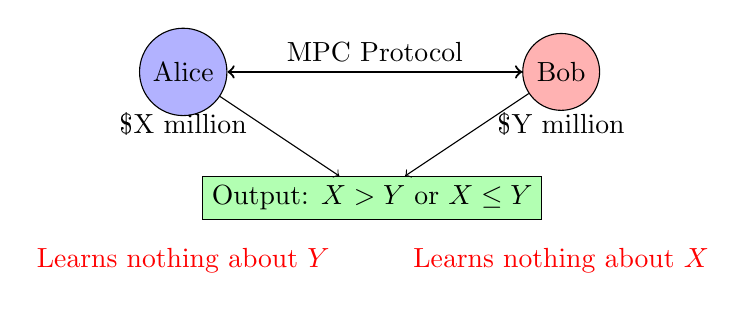
\begin{tikzpicture}[scale=0.8]
    % Alice
    \node[circle, draw, fill=blue!30] (alice) at (0,0) {Alice};
    \node[below] at (0,-0.5) {\$X million};

    % Bob
    \node[circle, draw, fill=red!30] (bob) at (6,0) {Bob};
    \node[below] at (6,-0.5) {\$Y million};

    % Protocol
    \draw[<->, thick] (alice) -- node[above] {MPC Protocol} (bob);

    % Result
    \node[draw, rectangle, fill=green!30] (result) at (3,-2) {Output: $X > Y$ or $X \leq Y$};
    \draw[->] (alice) -- (result);
    \draw[->] (bob) -- (result);

    % Privacy
    \node[red] at (0,-3) {Learns nothing about $Y$};
    \node[red] at (6,-3) {Learns nothing about $X$};
\end{tikzpicture}
\caption{Secure multiparty computation: Alice and Bob jointly evaluate a comparison function, learning only the result while each party's private input remains hidden from the other.}
\label{fig:ch16-mpc}
\end{figure}

\begin{definition}[Secure Computation]
\label{def:mpc}
A protocol $\Pi$ among $n$ parties securely computes $f$ if, for any adversary corrupting up to $t$ parties, there exists a simulator $S$ such that the adversary's view in $\Pi$ is computationally indistinguishable from $S$'s output given only the corrupted parties' inputs and the function output.
\end{definition}


\subsection{Shamir Secret Sharing}
\label{subsec:shamir}

The foundation of most MPC protocols is \emph{secret sharing}\index{secret sharing}: distributing a secret among $n$ parties so that any $t+1$ can reconstruct it, but any $t$ learn nothing.

\begin{definition}[Shamir's $(t+1, n)$-Secret Sharing]
\label{def:shamir}
To share a secret $s \in \Zq$:
\begin{enumerate}
\item Choose random coefficients $a_1, \ldots, a_t \getsr \Zq$.
\item Define the polynomial $p(x) = s + a_1 x + \cdots + a_t x^t \pmod{q}$.
\item Give party $i$ the share $s_i = p(i)$ for $i = 1, \ldots, n$.
\end{enumerate}
Any $t+1$ shares determine $p$ uniquely by Lagrange interpolation; any $t$ shares are uniformly distributed and reveal nothing about~$s$.
\end{definition}

Shamir secret sharing is information-theoretically secure---its security does not rely on any computational assumption and therefore survives quantum computers without modification.

\begin{svgraybox}
\textbf{Secret sharing as a hologram.}
In holography, every fragment of a holographic plate contains information about the entire image, but the image can only be reconstructed from enough fragments.  Shamir shares behave analogously: each share individually is uniformly random (contains no information about the secret), yet any sufficiently large collection of shares perfectly reconstructs the original.
\end{svgraybox}


\subsection{Garbled Circuits}
\label{subsec:garbled-circuits}

Yao's \emph{garbled circuits}\index{garbled circuits} protocol provides a general method for two-party secure computation:

\begin{enumerate}
\item The \emph{garbler} (Alice) takes the Boolean circuit for $f$, assigns random cryptographic labels to each wire's $0$ and $1$ values, and creates an encrypted truth table for each gate.
\item Alice sends the garbled circuit plus labels for her own input bits.
\item Bob obtains labels for his input bits via \emph{oblivious transfer} (OT)\index{oblivious transfer}---a sub-protocol in which Alice sends one of two values and learns nothing about Bob's choice, while Bob learns only his chosen value.
\item Bob evaluates the garbled circuit gate by gate and obtains labels for the output wires, which Alice helps decode.
\end{enumerate}

The security of garbled circuits reduces to the security of the symmetric encryption used for the truth tables and the security of oblivious transfer.


\subsection{MPC from Lattice-Based Oblivious Transfer}
\label{subsec:lattice-ot}

Oblivious transfer is the critical building block.  Classical OT protocols rely on the Diffie--Hellman assumption or RSA, both quantum-vulnerable.  Post-quantum OT can be constructed from the \lwe{} assumption:

\begin{enumerate}
\item The receiver generates an \lwe{} public key that encodes their choice bit $b \in \{0,1\}$.
\item The sender encrypts both messages $m_0, m_1$ under keys derived from the receiver's public key, such that only $m_b$ is decryptable.
\item The receiver decrypts $m_b$; the \lwe{} assumption guarantees that $m_{1-b}$ is computationally hidden.
\end{enumerate}

This \lwe{}-based OT, combined with garbled circuits, yields a complete post-quantum two-party computation protocol.  Extension to $n$ parties uses standard techniques (e.g., the BMR protocol or SPDZ with lattice-based preprocessing).

\begin{table}[t]
\caption{Post-quantum MPC overhead compared to classical MPC}
\label{tab:pq-mpc}
\begin{tabular}{p{3.5cm}p{2.5cm}p{2.5cm}p{2cm}}
\hline\noalign{\smallskip}
\textbf{Operation} & \textbf{Classical} & \textbf{Post-quantum} & \textbf{Overhead} \\
\noalign{\smallskip}\svhline\noalign{\smallskip}
AES evaluation & 13 ms & 18 ms & 1.4$\times$ \\
$10^6$ AND gates & 1.2 s & 2.1 s & 1.75$\times$ \\
ML inference & 5 s & 8 s & 1.6$\times$ \\
\noalign{\smallskip}\hline
\end{tabular}
\end{table}

The overhead of post-quantum MPC (Table~\ref{tab:pq-mpc}) is modest: typically 1.4--1.8$\times$ compared to classical protocols.  The bottleneck is the larger ciphertext and key sizes of lattice-based OT, not any fundamental efficiency barrier.


%% ================================================================
\section{Lattice-Based Advanced Constructions}
\label{sec:lattice-advanced}

The three primitives above---FHE, zero-knowledge proofs, and MPC---are general-purpose tools.  But the algebraic richness of lattices, particularly the trapdoor and preimage-sampling techniques developed by Gentry, Peikert, and Vaikuntanathan, enables a family of \emph{structured} primitives that control access to encrypted data in ways no other post-quantum assumption can match.  These constructions share a common mechanism: embedding access-control logic into the lattice structure itself, so that the ability to decrypt depends on algebraic relationships between keys, identities, attributes, or functions.  We survey four such constructions, in order of increasing generality.


\subsection{Identity-Based Encryption}
\label{subsec:ibe}

Public-key encryption as deployed today requires a cumbersome scaffolding: every user generates a key pair, a certificate authority vouches that a given public key belongs to a given person, and relying parties must validate these certificates before encrypting.  \emph{Identity-based encryption}\index{identity-based encryption} (IBE) collapses this machinery.  A user's public key \emph{is} their identity---an email address, a phone number, any unique string---and a trusted authority issues corresponding secret keys on demand.  The concept dates to Shamir (1984), but efficient constructions had to wait for lattice trapdoors.

The lattice realisation works as follows.  A master authority generates a random matrix $\mathbf{A} \in \Zq^{n \times m}$ together with a short basis (trapdoor) for the lattice $\lat^\perp(\mathbf{A})$.  When a user with identity $\mathit{id}$ requests a key, the authority applies the trapdoor to sample a short vector $\mathbf{s}$ satisfying $H(\mathit{id}) \cdot \mathbf{s} = \mathbf{0} \pmod{q}$, where $H$ is a public function mapping identities to matrices.  Anyone who wishes to encrypt a message to $\mathit{id}$ simply uses $H(\mathit{id})$ as the public key; the \lwe{} assumption guarantees that only the holder of $\mathbf{s}$ can decrypt.  Lattice IBE achieves \emph{adaptive} security under standard \lwe{} assumptions---a stronger guarantee than the pairing-based schemes it replaces, and one that survives quantum adversaries.


\subsection{Attribute-Based Encryption}
\label{subsec:abe}

IBE binds decryption to a single identity string.  In practice, access control is rarely that simple: a classified document should be readable by anyone in the Physics department with Secret clearance, regardless of individual identity.  \emph{Attribute-based encryption}\index{attribute-based encryption} (ABE) generalises IBE to handle exactly this kind of Boolean policy.  Ciphertexts carry attributes (``Department = Physics'', ``Clearance = Secret''), and decryption keys encode policies (``Department = Physics \textbf{AND} Clearance $\geq$ Secret'').  Decryption succeeds if and only if the ciphertext's attributes satisfy the key's policy---and the encryptor need not even know who will eventually decrypt.

\begin{definition}[Ciphertext-Policy ABE]
\label{def:cp-abe}
A ciphertext-policy ABE scheme consists of:
\begin{itemize}
\item $\mathsf{Setup}(\lambda) \to (\mathit{mpk}, \mathit{msk})$: Generate master public/secret keys.
\item $\Enc(\mathit{mpk}, P, m) \to \mathit{ct}$: Encrypt message $m$ under access policy~$P$.
\item $\KeyGen(\mathit{msk}, S) \to \mathit{sk}_S$: Issue a secret key for attribute set~$S$.
\item $\Dec(\mathit{sk}_S, \mathit{ct}) \to m$: Decrypt if and only if $S$ satisfies~$P$.
\end{itemize}
\end{definition}

Figure~\ref{fig:ch16-abe} illustrates the access-control mechanism: a document encrypted under the policy ``Physicist \textbf{AND} Q-Cleared'' can be decrypted only by a user whose attribute set satisfies both conditions.

\begin{figure}[t]
\centering
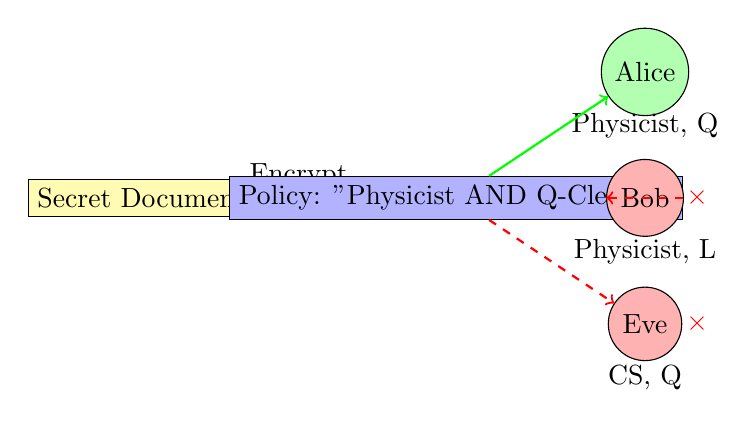
\begin{tikzpicture}[scale=0.8]
    % Document
    \node[draw, rectangle, fill=yellow!30] (doc) at (0,0) {Secret Document};

    % Encryption
    \draw[->, thick] (2,0) -- (3,0);
    \node[above] at (2.5,0) {Encrypt};

    % Policy
    \node[draw, rectangle, fill=blue!30] (policy) at (5,0) {Policy: "Physicist AND Q-Cleared"};

    % Different users
    \node[circle, draw, fill=green!30] (user1) at (8,2) {Alice};
    \node[below] at (8,1.5) {Physicist, Q};
    \draw[->, thick, green] (policy) -- (user1);
    \node[right, green] at (8.5,2) {\checkmark};

    \node[circle, draw, fill=red!30] (user2) at (8,0) {Bob};
    \node[below] at (8,-0.5) {Physicist, L};
    \draw[->, thick, red, dashed] (policy) -- (user2);
    \node[right, red] at (8.5,0) {$\times$};

    \node[circle, draw, fill=red!30] (user3) at (8,-2) {Eve};
    \node[below] at (8,-2.5) {CS, Q};
    \draw[->, thick, red, dashed] (policy) -- (user3);
    \node[right, red] at (8.5,-2) {$\times$};
\end{tikzpicture}
\caption{Attribute-based encryption: fine-grained access control through encryption.  Only users whose attributes satisfy the ciphertext policy can decrypt; others---even those holding a valid key for different attributes---learn nothing about the plaintext.}
\label{fig:ch16-abe}
\end{figure}

The lattice realisation of ABE rests on the technique of \emph{attribute-encoding} lattice trapdoors, introduced by Gentry, Sahai, and Waters.  The idea is to embed the policy evaluation directly into the lattice structure: each attribute contributes a matrix, and the policy determines how these matrices combine.  A user whose attribute set satisfies the policy can, through the algebraic structure, reconstruct a short vector that enables decryption; a user whose attributes fall short cannot, because the corresponding lattice problem remains hard.  Current lattice-based ABE constructions support policies expressible as Boolean formulas or even arbitrary circuits, though ciphertext and key sizes grow with policy complexity---the main barrier to deployment.


\subsection{Threshold Signatures and Distributed Key Generation}
\label{subsec:threshold}

A single compromised signing key can be catastrophic: a stolen certificate-authority key undermines every certificate it ever issued, and a stolen cryptocurrency wallet key drains the account irreversibly.  \emph{Threshold signatures}\index{threshold signature} eliminate this single point of failure by distributing signing authority among $n$ parties so that any $t+1$ can jointly produce a valid signature, but $t$ or fewer---even if fully corrupted---cannot sign at all.

For classical schemes like ECDSA, threshold protocols are well understood.  Lattice-based signatures introduce a complication that has no classical analogue: the signing process involves sampling from a discrete Gaussian distribution, and the noise in the resulting signature must fall within tight bounds for verification to succeed.  When signing is distributed, each party contributes a partial signature with its own noise, and the combined noise must still satisfy the global bound.  Achieving this requires \emph{distributed Gaussian sampling} protocols---each party samples locally, the partial samples are combined, and a rejection-sampling step ensures the aggregate has the correct distribution without leaking information about individual shares.  Recent constructions build on Shamir-style secret sharing of the lattice signing key, combined with these distributed sampling techniques, to achieve threshold variants of both Dilithium-style (Fiat--Shamir with aborts) and Falcon-style (NTRU trapdoor) signatures.  The main remaining obstacle is round complexity: current protocols require more interaction rounds than their classical counterparts.


\subsection{Functional Encryption}
\label{subsec:fe}

IBE and ABE control \emph{who} can decrypt.  \emph{Functional encryption}\index{functional encryption} (FE) goes further: it controls \emph{what} the decryptor learns.  A decryption key $\mathit{sk}_f$, associated with a function~$f$, allows its holder to compute $f(m)$ from a ciphertext encrypting~$m$---and nothing beyond $f(m)$.  Where ABE is an access-control mechanism, FE is an information-control mechanism: even authorised parties see only the specific derived quantity they need.

\begin{example}[Inner-Product Functional Encryption]
\label{ex:ipfe}
A hospital encrypts a patient record $\mathbf{m} \in \Zq^n$.  A researcher holds a key $\mathit{sk}_{\mathbf{y}}$ for a vector $\mathbf{y}$.  Decryption yields the inner product $\ip{\mathbf{m}}{\mathbf{y}} \pmod{q}$---e.g., a weighted health score---without revealing any other component of $\mathbf{m}$.  Lattice-based inner-product FE is efficient and secure under standard \lwe{} assumptions.
\end{example}

The gap between theory and practice in functional encryption is wide.  For restricted function classes---inner products and, more recently, degree-two polynomials---lattice-based constructions are efficient enough for deployment in privacy-preserving data analytics.  For arbitrary functions, FE constructions exist but rely on indistinguishability obfuscation, a primitive that is itself barely practical.  The frontier of FE research is therefore about pushing the boundary of ``which function classes can we support efficiently?''---a question where lattice techniques have made the most progress and are likely to continue leading.

These four constructions span a wide range of maturity, from deployed systems to active research frontiers.  Table~\ref{tab:advanced-maturity} summarises the current state.  FHE is the clear leader: the theory is settled and multiple production libraries exist, with performance as the remaining bottleneck.  IBE and threshold signatures have mature theoretical foundations and working prototypes, but deployment is limited by key-management complexity and round costs respectively.  ABE has strong theoretical results but faces a practical barrier in ciphertext and key sizes that grow with policy complexity.  Functional encryption for general functions remains the most open problem---a frontier where even the theoretical foundations are incomplete.

\begin{table}[t]
\caption{Maturity of lattice-based advanced constructions}
\label{tab:advanced-maturity}
\begin{tabular}{p{3.5cm}p{2.5cm}p{2.5cm}p{3cm}}
\hline\noalign{\smallskip}
\textbf{Primitive} & \textbf{Theory} & \textbf{Practice} & \textbf{Main challenge} \\
\noalign{\smallskip}\svhline\noalign{\smallskip}
FHE & Mature & Deployed & Performance \\
IBE & Mature & Prototypes & Key management \\
ABE & Mature & Research & Ciphertext/key size \\
Threshold signatures & Active & Prototypes & Distributed sampling \\
Functional encryption & Partial & Limited & General functions \\
\noalign{\smallskip}\hline
\end{tabular}
\end{table}


\section{Cryptography for Machine Learning}
\label{sec:crypto-ml}

\index{machine learning!cryptographic protection}
The advanced primitives surveyed in this chapter---FHE, zero-knowledge proofs, MPC, and the lattice-based constructions above---were developed to protect \emph{data}.  But the most valuable digital assets of the current decade are not databases or documents; they are trained machine-learning models.  A large language model may cost tens of millions of dollars to train, yet it can be queried through an API that, without cryptographic protection, leaks enough information for an adversary to reconstruct the model, poison its behaviour, or extract the private data on which it was trained.  The intersection of cryptography and machine learning is no longer a curiosity---it is a pressing deployment problem, and the primitives introduced earlier in this chapter are its primary tools.

\subsection{The Threat Landscape}
\label{subsec:ml-threats}

\index{model stealing}\index{adversarial examples}\index{training data extraction}
Four classes of attack define the threat model for deployed ML systems, and each admits a cryptographic defence:

\textbf{Model stealing.}  An adversary with query access to a model submits carefully chosen inputs and observes the outputs.  With enough queries---often surprisingly few---the adversary can train a surrogate model that approximates the original with high fidelity.  The economic damage is direct: the adversary obtains a multi-million-dollar model for the cost of API calls.  Cryptographic defence: \emph{secure inference} via FHE or MPC, where the model's internal computations are never exposed to the querier, even in encrypted form.  The FHE-based approach (Sect.~\ref{sec:fhe}) encrypts the model weights and evaluates the neural network homomorphically on encrypted inputs; the querier receives only the encrypted output, which it decrypts with its own key.  Current FHE-based inference is practical for small models (logistic regression, decision trees, shallow networks) but remains prohibitively slow for large transformer architectures---a gap that bootstrapping improvements are steadily closing.

\textbf{Data poisoning and adversarial examples.}  An adversary who can inject malicious samples into the training set can embed hidden triggers (backdoors) that cause the model to behave predictably on attacker-chosen inputs while performing normally on clean data.  At inference time, adversarial examples---inputs crafted to fool the model into misclassification---exploit the same fragility from a different angle.  Cryptographic defence: \emph{verified training} via zero-knowledge proofs (Sect.~\ref{sec:zkp}).  The model trainer produces a ZK proof that the training process followed a specified protocol on a committed dataset, without revealing the data itself.  Verifiers can check the proof to confirm that no poisoning occurred.  For adversarial robustness at inference time, \emph{cryptographic commitments} can bind model outputs to specific inputs, enabling auditable predictions---though certified robustness against all adversarial perturbations remains an open problem at the intersection of optimisation theory and cryptography.

\textbf{Training data extraction.}  Large models memorise fragments of their training data, and targeted prompting can extract verbatim passages---including personally identifiable information, copyrighted text, or proprietary data that was never intended for disclosure.  Cryptographic defence: \emph{private learning} combines differential privacy\index{differential privacy} with cryptographic protocols.  Differential privacy injects calibrated noise during training so that no single training example significantly influences the model's outputs; MPC-based training (Sect.~\ref{sec:mpc}) allows multiple data holders to contribute training data without any party---including the model trainer---seeing another party's raw data.  The combination provides a formal privacy guarantee backed by both information-theoretic and computational assumptions.

Table~\ref{tab:ml-crypto-defences} summarises the mapping from ML attacks to cryptographic defences.

\begin{table}[t]
\caption{Cryptographic defences for machine-learning systems\index{machine learning!defence table}}
\label{tab:ml-crypto-defences}
\begin{tabular}{p{3cm}p{3.5cm}p{3cm}p{2.5cm}}
\hline\noalign{\smallskip}
\textbf{Attack class} & \textbf{Cryptographic defence} & \textbf{Primitive} & \textbf{Maturity} \\
\noalign{\smallskip}\svhline\noalign{\smallskip}
Model extraction & Secure inference & FHE, MPC & Prototypes \\
Data poisoning & Verified training & Zero-knowledge proofs & Research \\
Adversarial examples & Certified robustness & Commitments & Research \\
Privacy leakage & Private learning & DP + MPC & Deployed \\
\noalign{\smallskip}\hline
\end{tabular}
\end{table}


\subsection{AI-Assisted Cryptanalysis}
\label{subsec:ai-cryptanalysis}

\index{cryptanalysis!AI-assisted}
The relationship between cryptography and machine learning runs in both directions.  ML techniques are increasingly applied \emph{to} cryptanalysis, and post-quantum schemes are not immune.

Side-channel analysis was among the first beneficiaries.  Deep-learning classifiers trained on power or electromagnetic traces can recover secret keys from protected implementations with fewer traces than classical statistical methods (CPA, template attacks), because they learn non-linear leakage models that Hamming-weight assumptions miss~\cite{MaghrebiBrierDanger2019}.  For PQC hardware, this means that the masking-order calculations in Chapter~\ref{ch:hardware-security} are conservative: an ML-enhanced attacker may need fewer traces than the theoretically predicted minimum for a given masking order, particularly when the implementation has subtle leakage beyond the assumed power model.

Beyond side channels, ML is being applied to lattice cryptanalysis itself: learning lattice-sieving heuristics, optimising BKZ block strategies, and searching for structural weaknesses in new algebraic constructions.  The results so far are incremental---no ML-driven break of a NIST-standardised parameter set---but the trajectory suggests that ML will become a standard tool in the cryptanalyst's repertoire, accelerating the discovery of weaknesses and widening the gap between ``provably hard'' and ``hard in practice.''

The implication for post-quantum cryptography is a familiar one, stated with renewed force: security margins matter.  Parameter sets should be chosen not merely to resist today's best algorithms but to absorb the accelerating pace of both classical and ML-assisted cryptanalysis.  The lattice-reduction evolution documented in Table~\ref{tab:lattice-reduction-evolution} of Chapter~\ref{ch:hardware-security} illustrates the trend; ML-assisted optimisation is likely to steepen it.

The primitives in this chapter---FHE for secure inference, ZK proofs for verified computation, MPC for private training---are the building blocks of a future where machine-learning systems are both cryptographically protected and cryptographically accountable.  The constructions are mature enough for targeted deployment today; making them efficient enough for large-scale ML workloads is one of the most consequential open problems at the intersection of cryptography and computer science.


%% ================================================================
\section*{Problems}
\addcontentsline{toc}{section}{Problems}

\begin{prob}
\label{prob:ch14-fhe}
\textbf{FHE noise budget.}\\
In an \lwe{}-based FHE scheme, a fresh ciphertext has noise magnitude $\sigma$.  After one homomorphic multiplication, the noise grows to approximately $\sigma^2 \cdot n$ where $n$ is the lattice dimension.  If the modulus is $q$ and decryption fails when noise exceeds $q/2$:
\begin{enumerate}
\item[(a)] Show that after $L$ levels of multiplication the noise is approximately $\sigma^{2^L} \cdot n^{2^L - 1}$.
\item[(b)] Derive the maximum multiplicative depth $L_{\max}$ as a function of $\sigma$, $n$, and $q$ by solving $\sigma^{2^L} \cdot n^{2^L - 1} = q/2$.
\item[(c)] For $\sigma = 3.2$, $n = 1024$, $q = 2^{27}$, compute $L_{\max}$.  How many multiplications can be performed before bootstrapping is required?
\end{enumerate}
\end{prob}

\begin{prob}
\label{prob:ch14-zkp}
\textbf{Stern-type soundness.}\\
A Stern-type zero-knowledge protocol has soundness error $2/3$ per round.
\begin{enumerate}
\item[(a)] How many rounds are needed to achieve soundness error below $2^{-128}$?
\item[(b)] If each round requires sending three commitments of 256~bits each, estimate the total proof size.
\item[(c)] The Fiat--Shamir transform converts this interactive proof into a non-interactive one.  In the quantum random oracle model, the soundness loss is a multiplicative factor of $\sqrt{q_H}$ where $q_H$ is the number of hash queries.  If we allow $q_H = 2^{64}$ quantum queries, how many additional rounds must be added to maintain $2^{-128}$ soundness?
\end{enumerate}
\end{prob}

\begin{prob}
\label{prob:ch14-shamir}
\textbf{Secret sharing arithmetic.}\\
Consider Shamir $(3, 5)$-secret sharing over $\Z_{17}$.  The dealer wishes to share $s = 11$.
\begin{enumerate}
\item[(a)] Choose random coefficients $a_1, a_2 \in \Z_{17}$ and compute the five shares.
\item[(b)] Verify that any three shares reconstruct $s$ via Lagrange interpolation.
\item[(c)] Verify that any two shares are consistent with \emph{every} possible secret $s' \in \Z_{17}$.
\item[(d)] Suppose two parties hold shares of secrets $s$ and $s'$ respectively (shared with the same evaluation points).  Explain how the parties can compute shares of $s + s'$ without interaction, and shares of $s \cdot s'$ with one round of communication.  Why does multiplication increase the threshold?
\end{enumerate}
\end{prob}

\begin{prob}
\label{prob:ch14-advanced}
\textbf{Research-level.}\\
Functional encryption for inner products over $\Zq$ allows a key holder to learn $\ip{\mathbf{m}}{\mathbf{y}}$ from an encryption of $\mathbf{m}$.  Explain why this does \emph{not} trivially allow recovery of $\mathbf{m}$ itself (even if the adversary can request keys for many different vectors $\mathbf{y}$), provided $\dim(\mathbf{m}) > $ the number of key queries.  What happens when the number of queries equals $\dim(\mathbf{m})$?  Discuss the implications for bounding the number of functional decryption keys in a practical deployment.
\end{prob}
